\subsubsection{Typ}
Servermodul som i huvudsak består av PHP-skript.

\subsubsection{Syfte}
Syftet med databehandlingsmodulen är att ta emot data från applikationstestaren i form av inspelade upplevelser av applikationen. Mottagen data innehåller, beroende på vad applikationstestaren spelat in; skärmdumpar, touch, ljud, inspelning från frontkameran samt diverse metadata om mobiltelefonen. Denna data sammanställs sedan där resultatet blir en film som sparas på servern samt data kring filmen och mobiltelefonen som sparas i en databas.

\subsubsection{Funktionalitet}
Data skickas från överföringsdelen via \texttt{HTTP}-protokollet genom metoden \texttt{POST} till servern där ett PHP-skript väntar. Mottagen data behandlas sedan av ett annat PHP-skript som använder submoduler för att sätta ihop skärmdumpar, touch, ljud och kamerainspelning till en video. Submodulerna returnerar en videofilm som sparas på servern. Till sist lagras information om videofilmen samt metadata från mobiltelefonen i en MySQL-databas.

\subsubsection{Underordnade komponenter}
Underordnade komponenter är \nameref{sub:touchmedia} och \nameref{sub:screenmedia}.

\subsubsection{Beroenden}
Denna modul kan komma att bero på PHP-ramverket Laravel. Databehandlingen skapas i mån av tid som en insticksmodul till Laravel vilket skapar ett beroende till ramverkets kärnfiler som då måste finnas på servern.

\subsubsection{Gränssnitt}
Denna modul har inget användargränssnitt utan jobbar med \texttt{HTTP}-protokollet mot överföringsdelen.

\subsubsection{Resurser}
För att över huvud taget kunna använda denna modul krävs en servermiljö som kan exekvera PHP-skript och som har tillgång till en MySQL-databas. Dessutom krävs lagringsutrymme på servern för att kunna spara videofilmerna.

\subsubsection{Referenser}
Sektion 2.3.5 i URD-1 ger en motivering till varför sammansättning av media sker på serversidan istället för i mobiltelefonen. Sektion 2.6 i URD-1 handlar om servermiljön och under 2.6.2 ges en kort förklaring programmet FFmpeg som kommer att användas vid databehandlingen.

\subsubsection{Process}
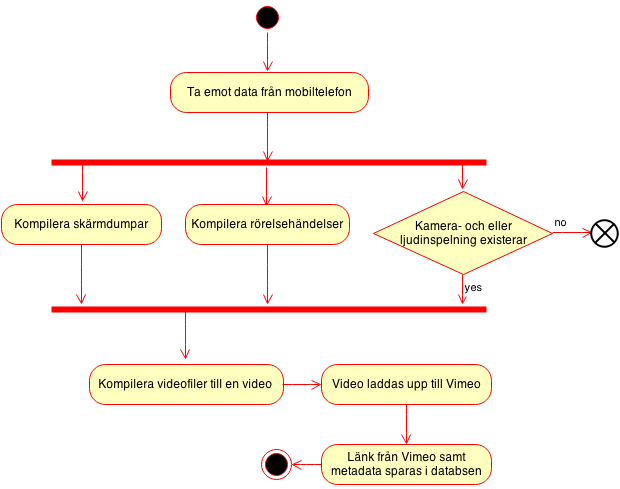
\includegraphics[scale=0.6]{dataprocessing.png}

\subsubsection{Data}
Den data som mottas från mobiltelefonen är en zip-fil innehållandes skärmdumpar, metadata samt rörelsehändelser och eventuell kamera- och ljudinspelning. När alla data har behandlats skickas den slutliga videofilen till Vimeo och endast metadata sparas på i databasen.
